  \subsection{Análisis de un tren de pulsos}

    Se setea la señal de entrada.

        \begin{figure}[H]
        \centering
        \begin{subfigure}[H]{0.48\textwidth}
          \frame{\includegraphics[width=\textwidth]{Imagenes/ActividadPractica/2AnalisisDeUnTrenDePulsos/Exp2_PeriodoDeLaSeñalDeEntrada.jpeg}}
          \caption{Señal pulsante de entrada, período de $1~ms$.}
        \end{subfigure}
        \hfill
        \begin{subfigure}[H]{0.48\textwidth}
          \frame{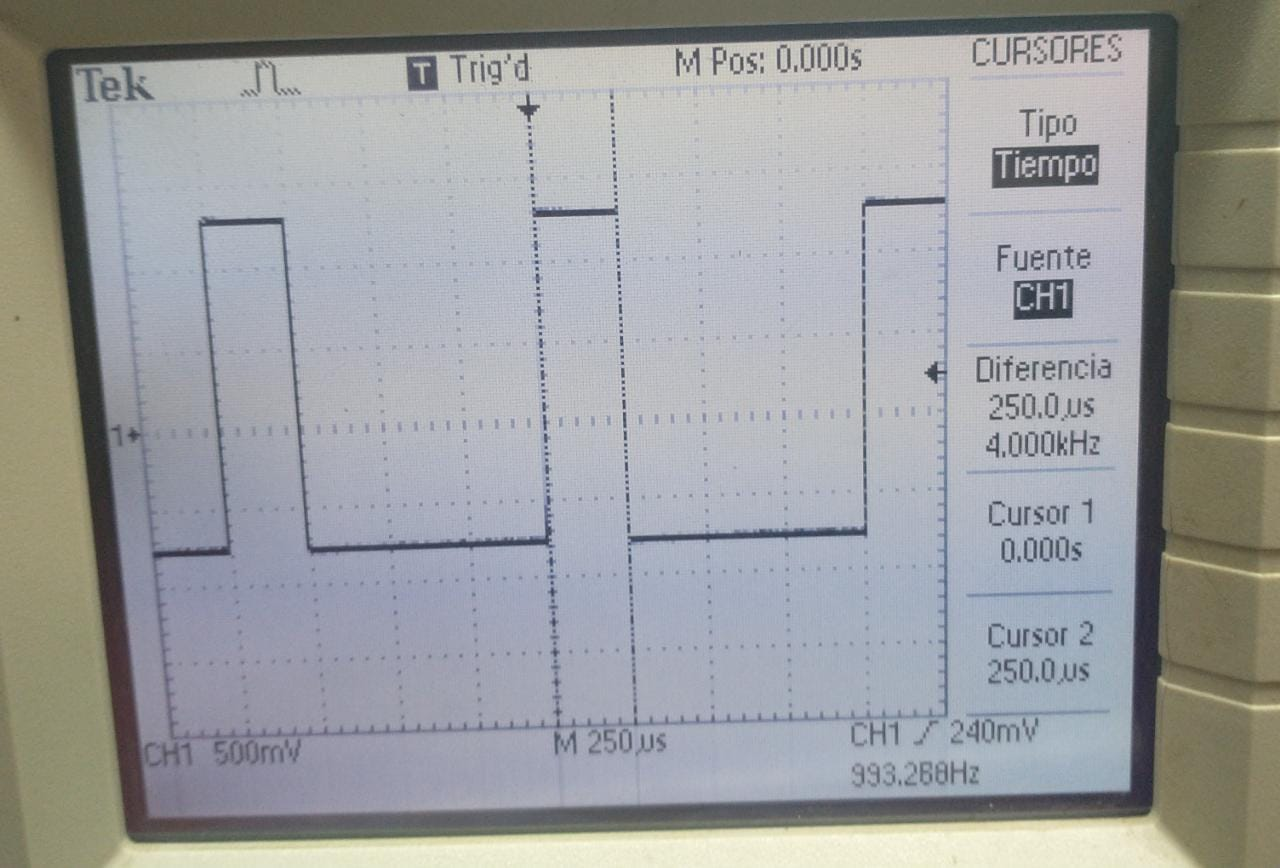
\includegraphics[width=\textwidth]{Imagenes/ActividadPractica/2AnalisisDeUnTrenDePulsos/Exp2_AnchoDelPulsoDeEntrada.jpeg}}
          \caption{Ancho del pulso.}
        \end{subfigure}

        \caption{Señal pulsante de entrada.}
        \label{fig:Exp2SeñalPulso}
      \end{figure}

    Se observa en el espectro.

      \begin{figure}[H]
        \centering
          \frame{\includegraphics[width=0.48\textwidth]{Imagenes/ActividadPractica/2AnalisisDeUnTrenDePulsos/Exp2_EspectroDeLaSeñalPulsante.jpeg}}
          \caption{Análisis en frecuencia de la señal de entrada.}
          \label{fig:Exp2SeñalPulsanteEspectro}
      \end{figure}

      Luego se conmuta en los tres tipos de ventana.

      \begin{figure}[H]
        \centering
        \begin{subfigure}[H]{0.48\textwidth}
          \frame{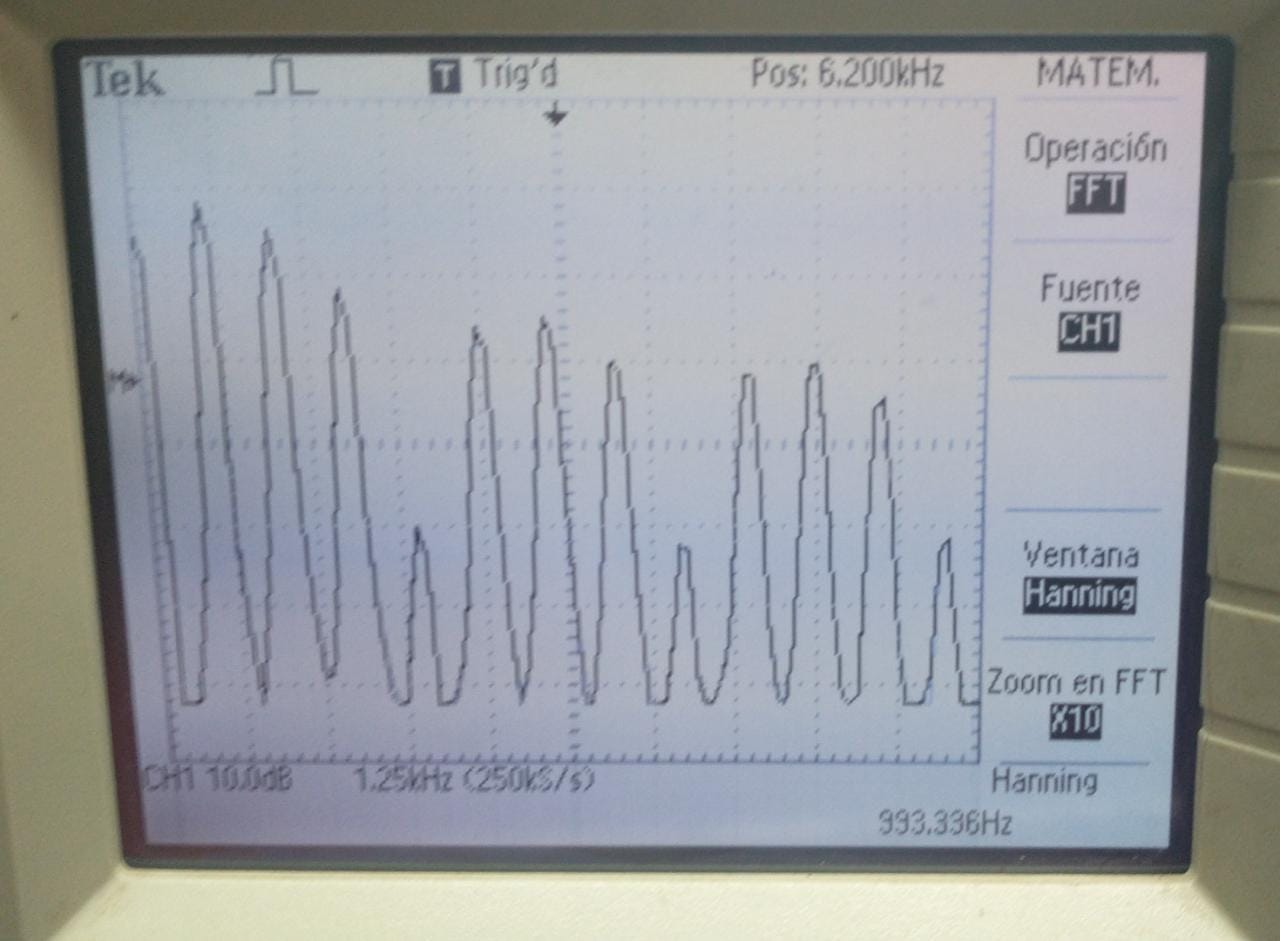
\includegraphics[width=\textwidth]{Imagenes/ActividadPractica/2AnalisisDeUnTrenDePulsos/Exp2_EspectroEnVentanaHannin.jpeg}}
          \caption{Análisis en frecuencia, ventana Hanning.}
        \end{subfigure}
        \hfill
        \begin{subfigure}[H]{0.48\textwidth}
          \frame{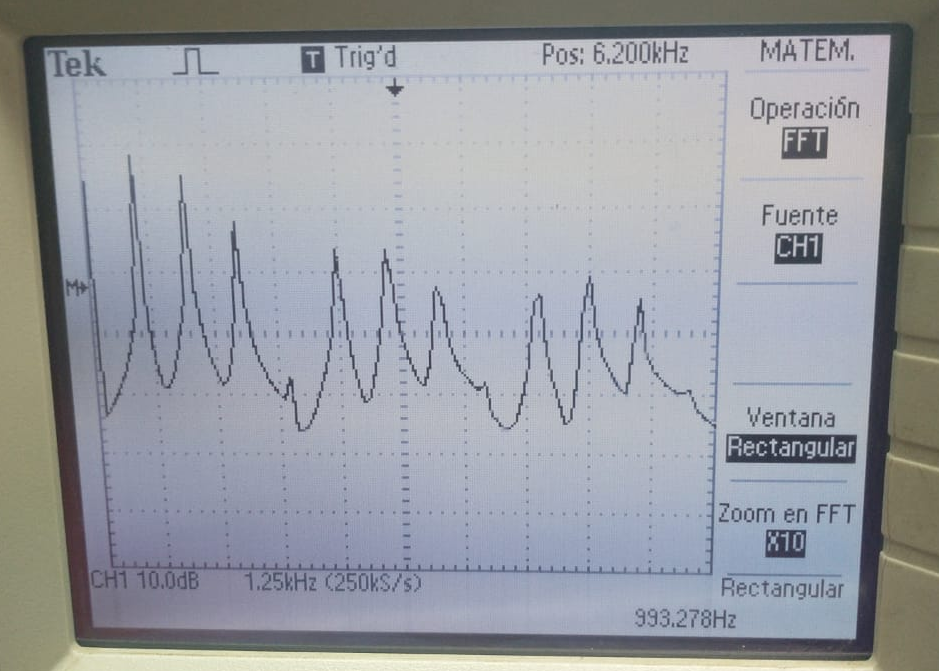
\includegraphics[width=\textwidth]{Imagenes/ActividadPractica/2AnalisisDeUnTrenDePulsos/Exp2_EspectroEnVentanaRectangular.png}}
          \caption{Análisis en frecuencia, ventana Rectangular.}
        \end{subfigure}
        \begin{subfigure}[H]{0.48\textwidth}
          \frame{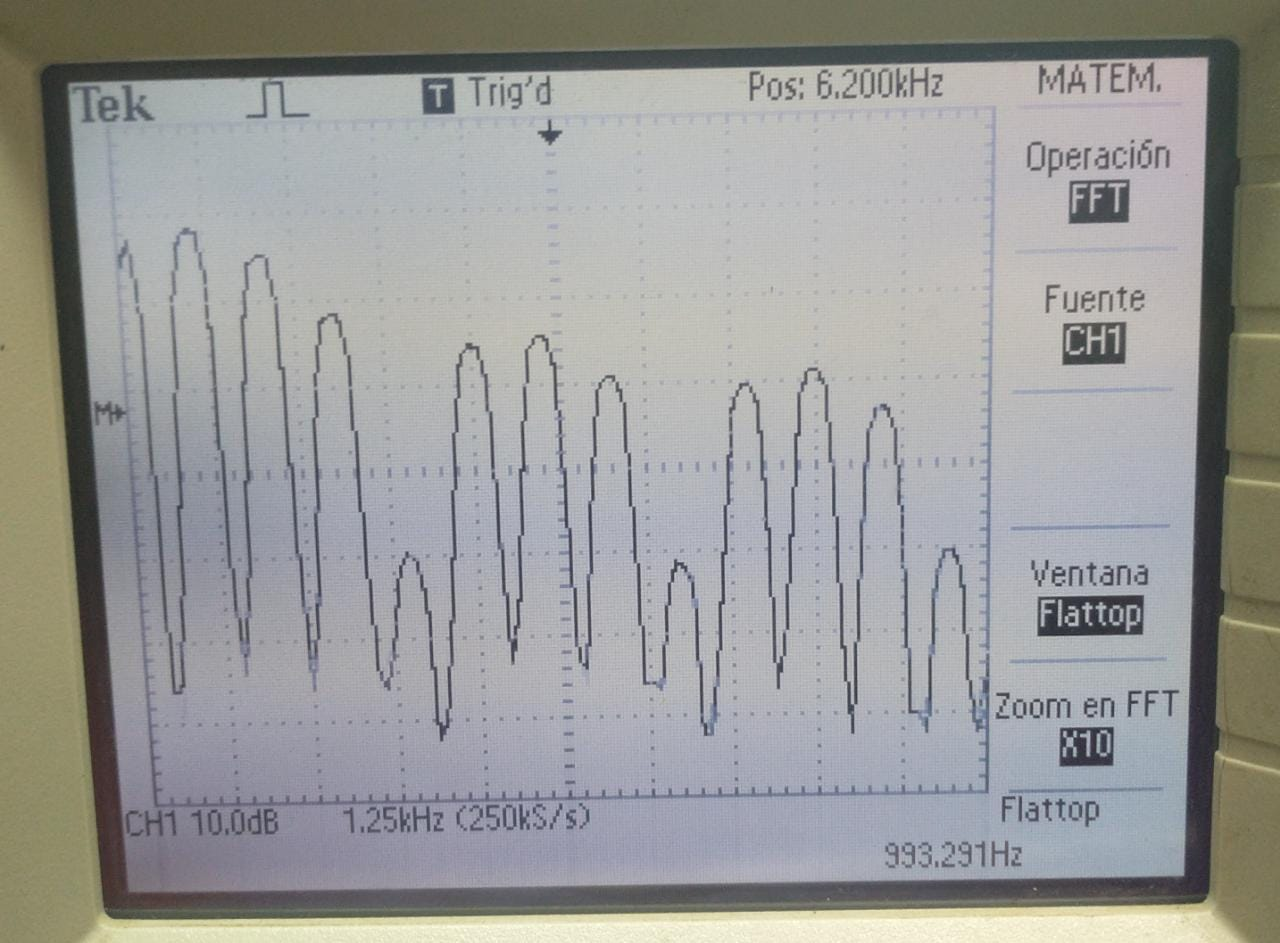
\includegraphics[width=\textwidth]{Imagenes/ActividadPractica/2AnalisisDeUnTrenDePulsos/Exp2_EspectroEnVentanaFlattop.jpeg}}
          \caption{Análisis en frecuencia, ventana Flattop.}
        \end{subfigure}

        \caption{Señal pulsante de entrada.}
        \label{fig:Exp2SeñalPulsanteVentanasEspectro}
      \end{figure}

      Se observan los 5 primeros armónicos en ventana Hanning.

       \begin{figure}[H]
        \centering
        \begin{subfigure}[H]{0.48\textwidth}
          \frame{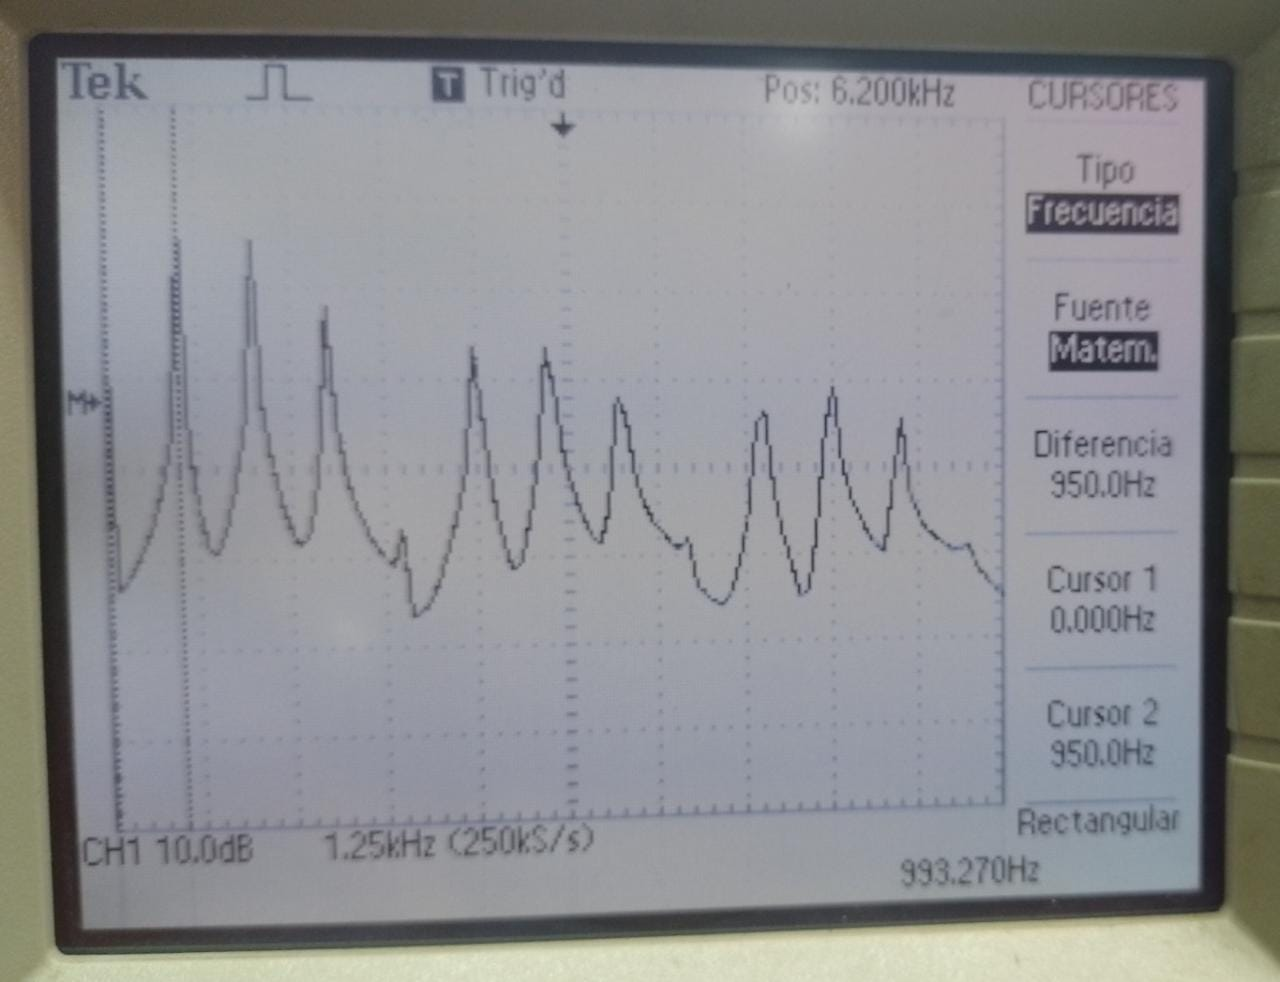
\includegraphics[width=\textwidth]{Imagenes/ActividadPractica/2AnalisisDeUnTrenDePulsos/Exp2_FrecArmonico1.jpeg}}
          \caption{Frecuencia de la fundamental en ventana Hanning, $f_{1}=950~Hz$.}
        \end{subfigure}
        \hfill
        \begin{subfigure}[H]{0.48\textwidth}
          \frame{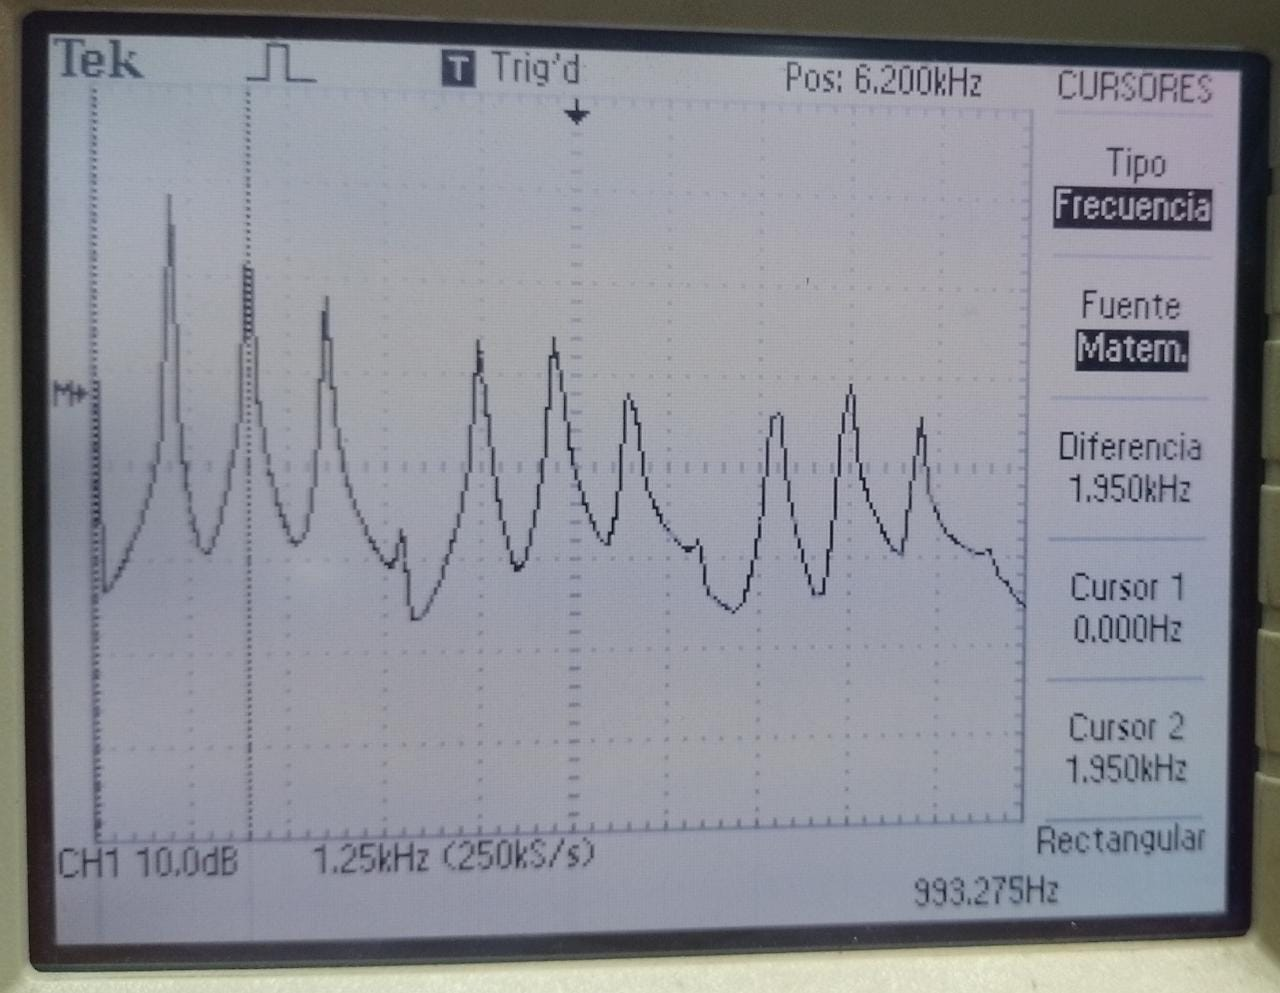
\includegraphics[width=\textwidth]{Imagenes/ActividadPractica/2AnalisisDeUnTrenDePulsos/Exp2_FrecArmonico2.jpeg}}
          \caption{Frecuencia de la segunda armónica en ventana Hanning, $f_{2}=1950~Hz$.}
        \end{subfigure}
        \begin{subfigure}[H]{0.48\textwidth}
          \frame{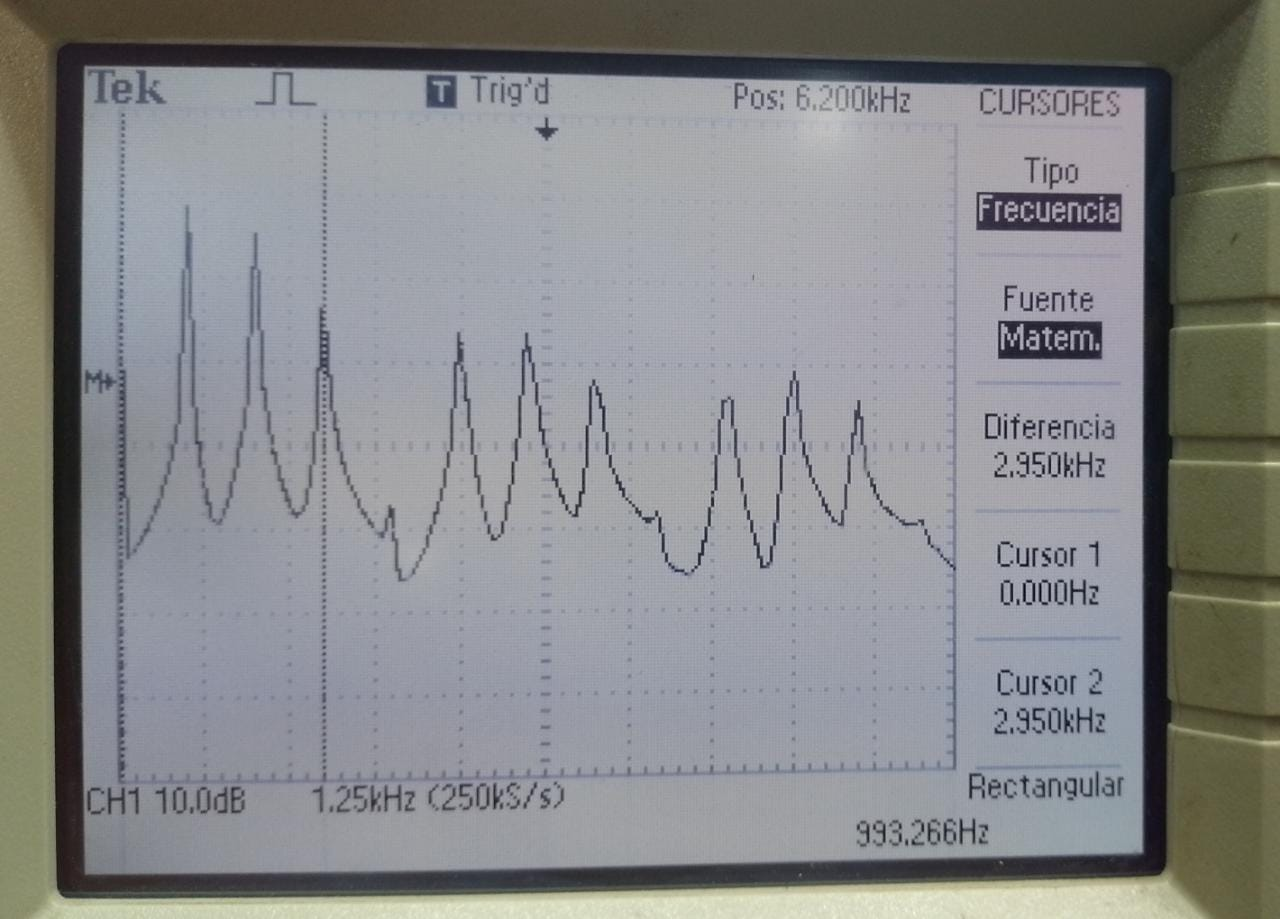
\includegraphics[width=\textwidth]{Imagenes/ActividadPractica/2AnalisisDeUnTrenDePulsos/Exp2_FrecArmonico3.jpeg}}
          \caption{Frecuencia de la tercera armónica en ventana Hanning, $f_{3}=2950~Hz$.}
        \end{subfigure}
        \begin{subfigure}[H]{0.48\textwidth}
          \frame{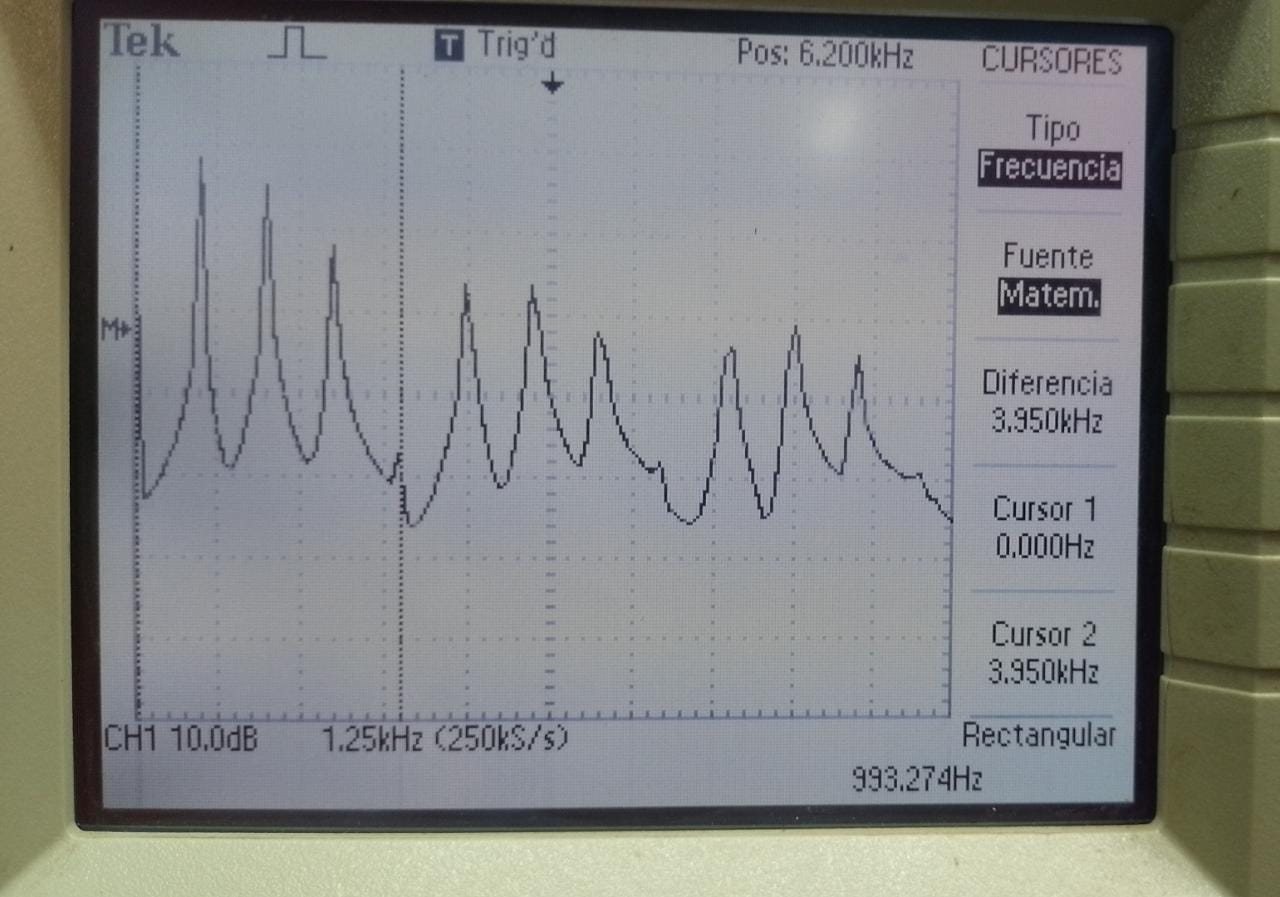
\includegraphics[width=\textwidth]{Imagenes/ActividadPractica/2AnalisisDeUnTrenDePulsos/Exp2_FrecArmonico4.jpeg}}
          \caption{Frecuencia de la cuarta armónica en ventana Hanning, $f_{4}=3950~Hz$.}
        \end{subfigure}
        \begin{subfigure}[H]{0.48\textwidth}
          \frame{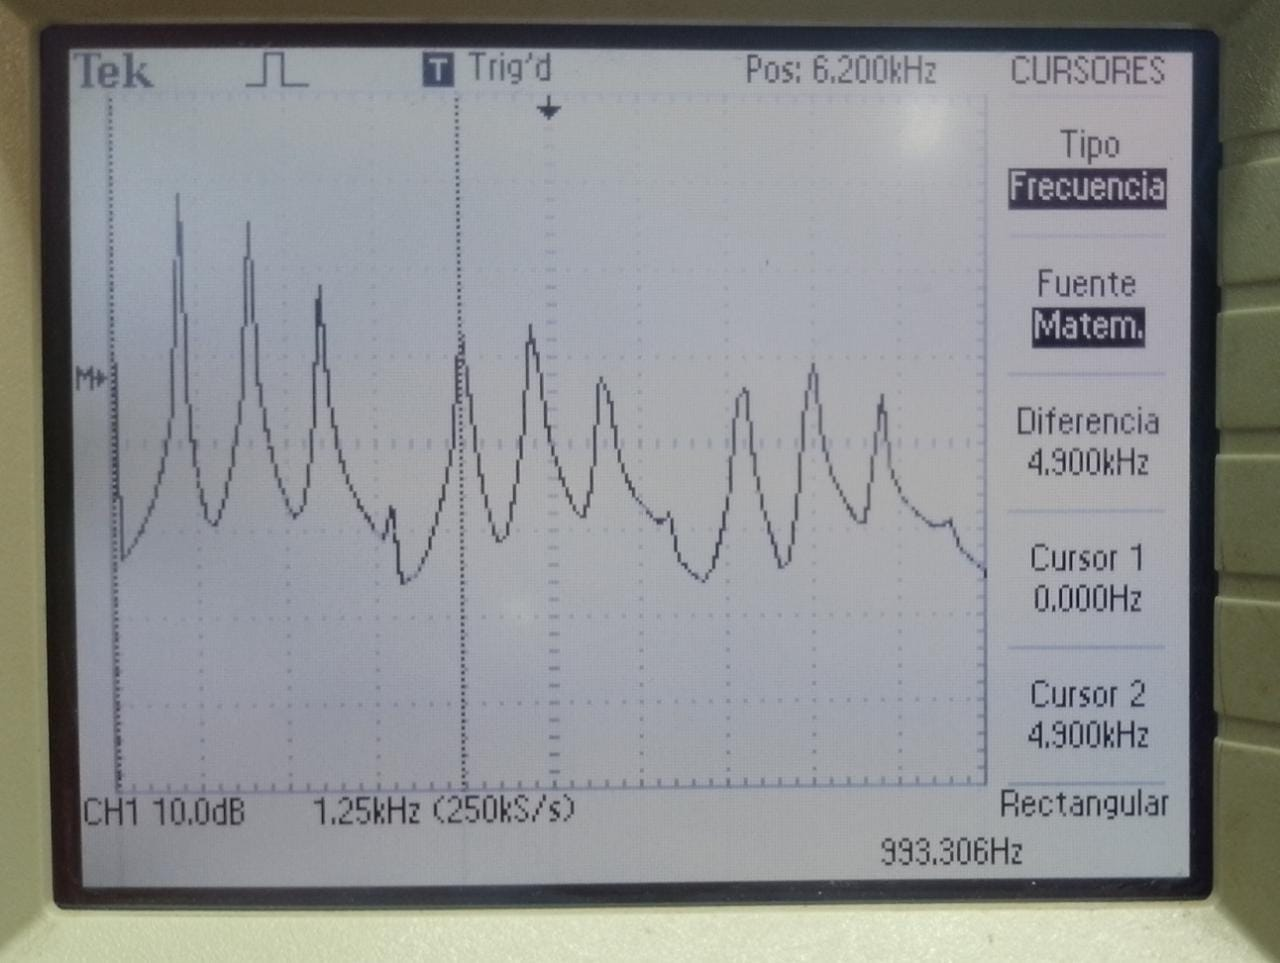
\includegraphics[width=\textwidth]{Imagenes/ActividadPractica/2AnalisisDeUnTrenDePulsos/Exp2_FrecArmonico5.jpeg}}
          \caption{Frecuencia de la quinta armónica en ventana Hanning, $f_{5}=4900~Hz$.}
        \end{subfigure}

        \caption{Medición de frecuencia de armónicos de la señal pulsante en ventana Hanning.}
        \label{fig:Exp2SeñalPulsanteArmonicosEspectro}
      \end{figure}     

      Luego se pasa a Flattop y se miden las frecuencias de los valles.

       \begin{figure}[H]
        \centering
        \begin{subfigure}[H]{0.48\textwidth}
          \frame{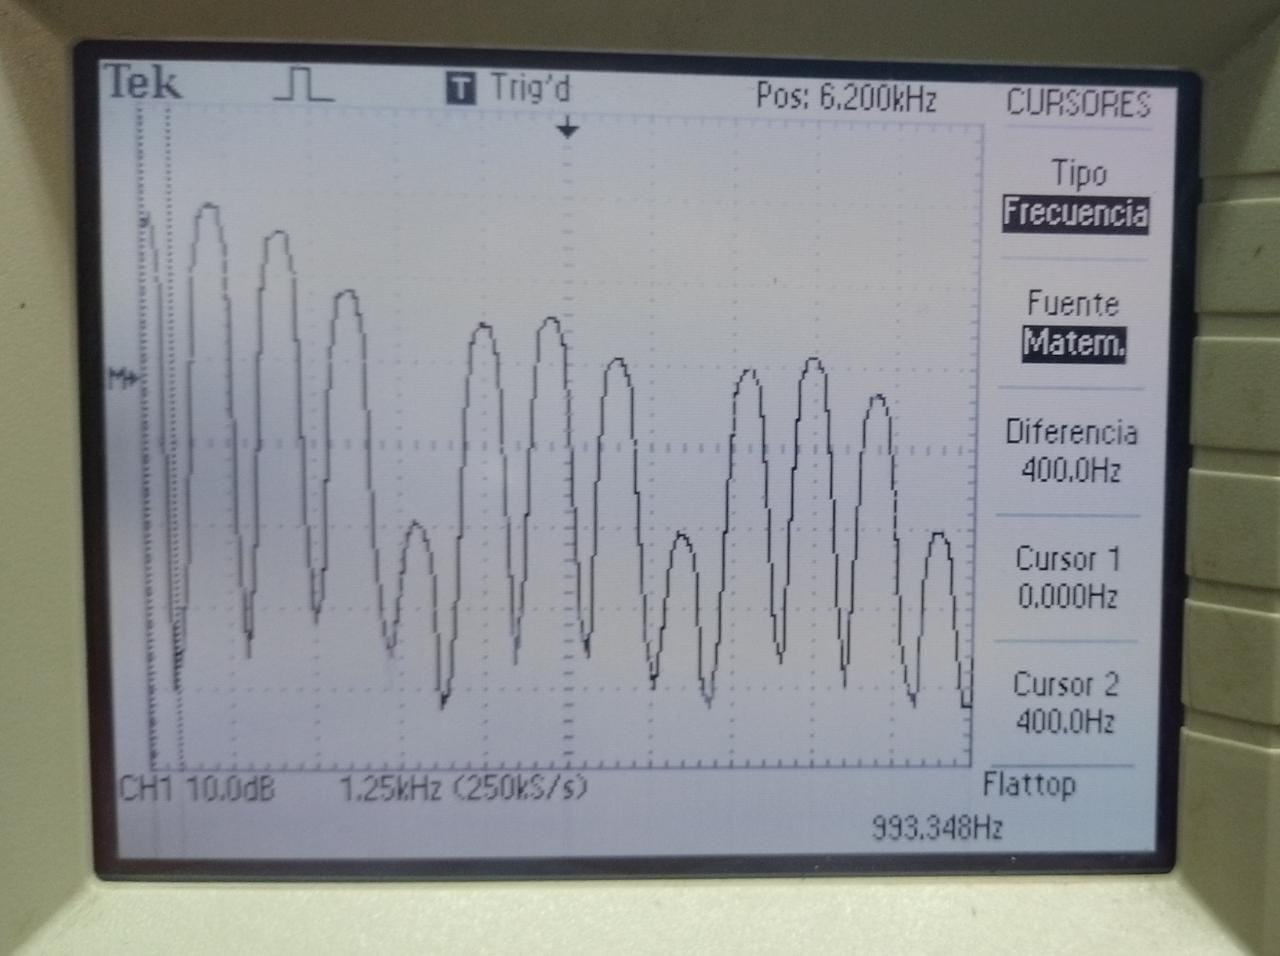
\includegraphics[width=\textwidth]{Imagenes/ActividadPractica/2AnalisisDeUnTrenDePulsos/Exp2_FrecValle1Flattop.jpeg}}
          \caption{Frecuencia del primer valle en ventana Flattop, $f_{a}=400~Hz$.}
        \end{subfigure}
        \hfill
        \begin{subfigure}[H]{0.48\textwidth}
          \frame{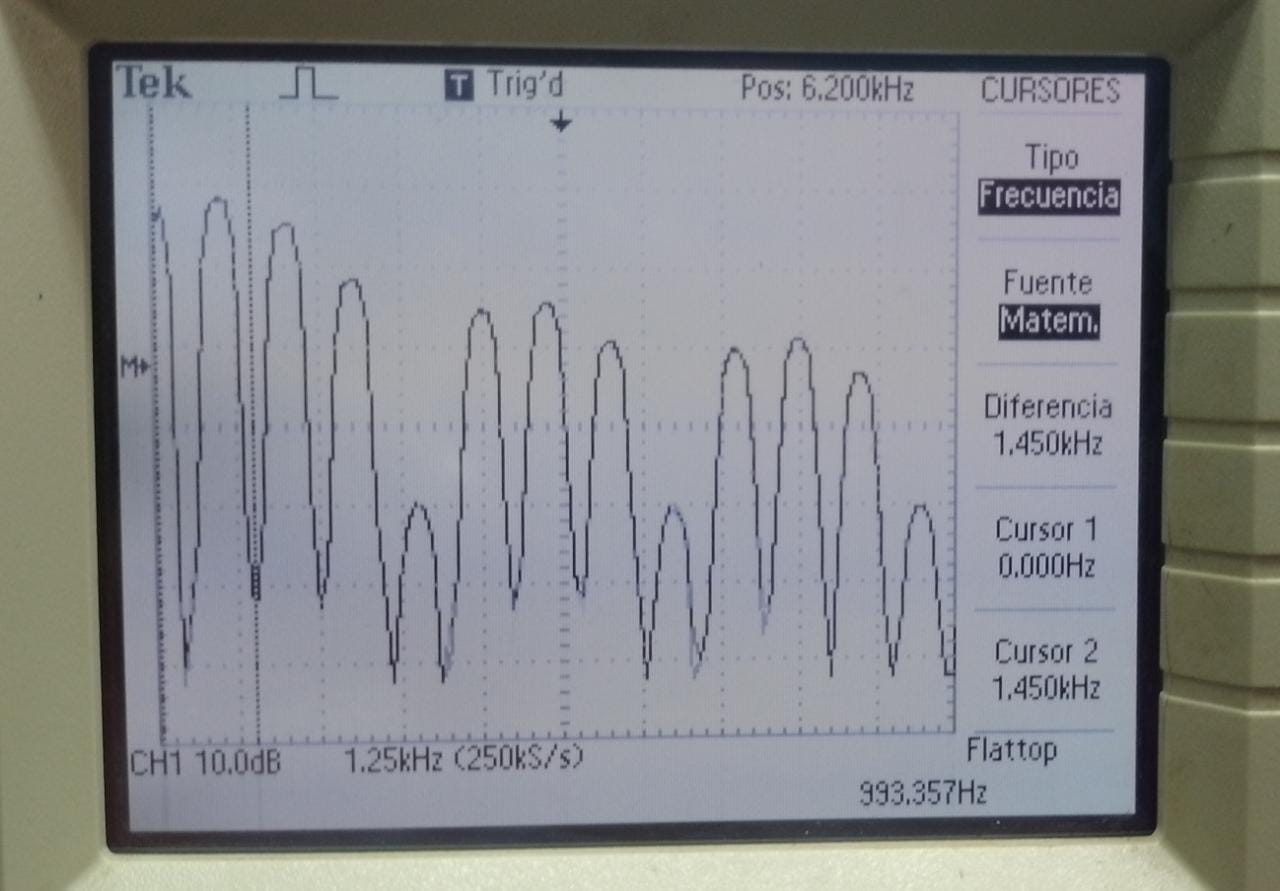
\includegraphics[width=\textwidth]{Imagenes/ActividadPractica/2AnalisisDeUnTrenDePulsos/Exp2_FrecValle2Flattop.jpeg}}
          \caption{Frecuencia del segundo valle en ventana Rectangular, $f_{b}=1450~Hz$.}
        \end{subfigure}
        \hfill
        \begin{subfigure}[H]{0.48\textwidth}
          \frame{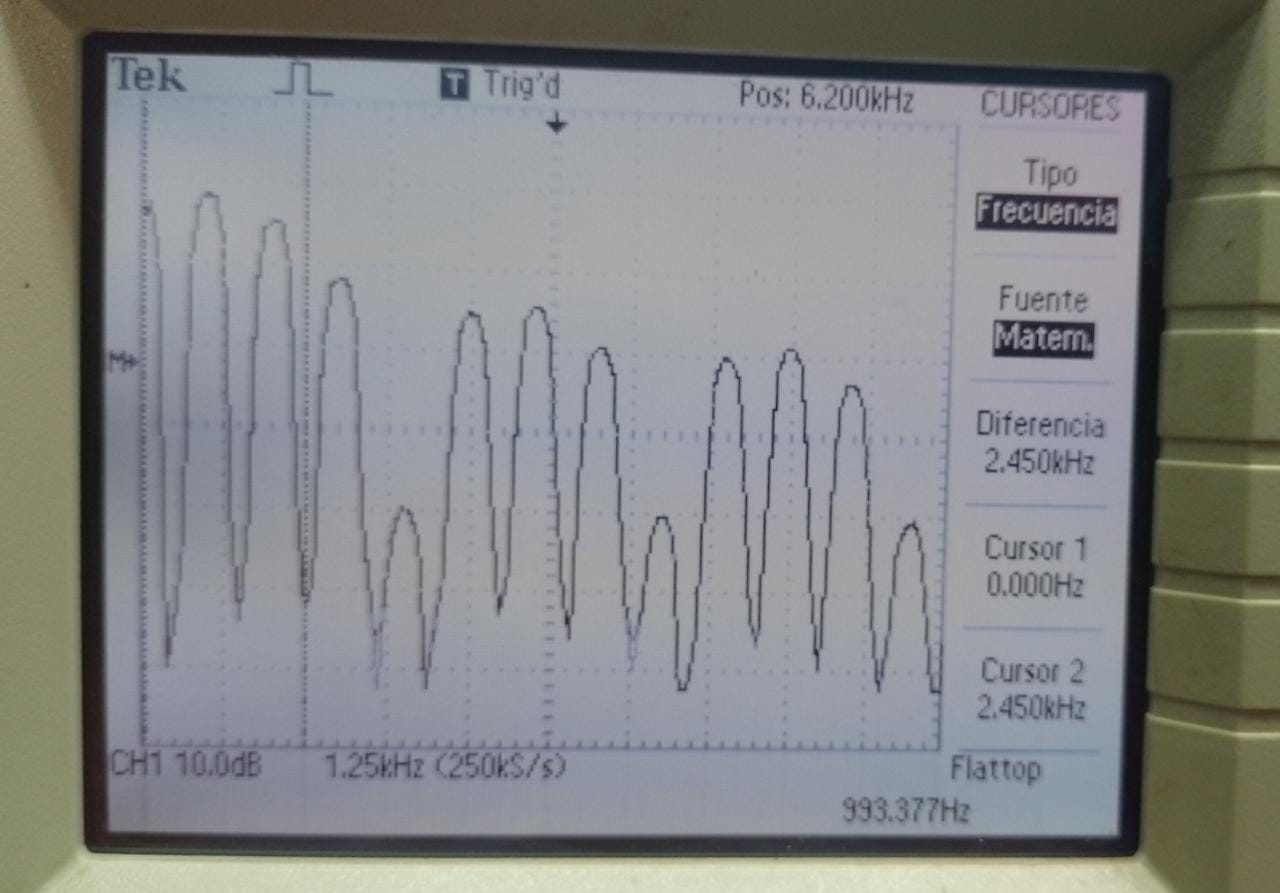
\includegraphics[width=\textwidth]{Imagenes/ActividadPractica/2AnalisisDeUnTrenDePulsos/Exp2_FrecValle3Flattop.jpeg}}
          \caption{Frecuencia del tercer valle en ventana Flattop, $f_{c}=2450~Hz$.}
        \end{subfigure}

        \caption{Medición de frecuencia de valles de la señal pulsante en ventana Flattop.}
        \label{fig:Exp2SeñalPulsanteVallesEspectro}
      \end{figure}     

      Se hace una tabla para la ventana Hanning. Se coloca el cursor 1 en 0Hz y el otro marca el 
      armónico.

      \begin{table}[H]
      \centering
        \begin{tabular}{cccccc} \hline \hline
          \textbf{Cursor 2}               &  $\mathbf{1erArm.}$       & $\mathbf{2daArm.}$        & $\mathbf{3raArm.}$  &   $\mathbf{4taArm.}$ &   $\mathbf{5taArm.}$ \\ \hline
          $\mathbf{\Delta_{fn}~Hz}$       &   $950$                        &    $950$                    &   $950$                & $950$                   & $950$                \\
         \end{tabular}
          \caption{Valores de frecuencia medidos en ventan Hanning.}
          \label{tab:Exp1MedicionesHanning}
      \end{table}

      Se calcula el promedio de las frecuencias.

      \begin{align*}
        \Delta_{fn_{prom}}=\dfrac{\sum{\Delta_{fn}}}{n} \hspace{20pt} \therefore \hspace{20pt} \boxed{\Delta_{fn_{prom}}=950~[Hz]}
      \end{align*}

      Y el período de la onda de pulsos es.

      \begin{align*}
        Periodo~\left( T \right)=\dfrac{1}{\Delta_{fn_{prom}}} \hspace{20pt} \therefore \hspace{20pt} \boxed{Periodo~\left( T \right)=1,053~[ms]}
      \end{align*}

      Se cambia a flattop y se miden los valles.

      \begin{table}[H]
      \centering
        \begin{tabular}{cccc} \hline \hline
          \textbf{Cursor 2}               &  $\mathbf{1erArm.}$       & $\mathbf{2daArm.}$        & $\mathbf{3raArm.}$   \\ \hline
          $\mathbf{\Delta_{fmin}~Hz}$       &   $400$                        &    $1050$                    &   $1000$                     \\
         \end{tabular}
          \caption{Valores de frecuencia medidos en ventan Flattop.}
          \label{tab:Exp1MedicionesFlattop}
      \end{table}  

      También se calcula promedio y período.

      \begin{align*}
        \Delta_{fn_{prom}}=\dfrac{\sum{\Delta_{fn}}}{n} \hspace{20pt} \therefore \hspace{20pt} \boxed{\Delta_{fn_{prom}}=816,67~[Hz]}
      \end{align*}        

      \begin{align*}
        Periodo~\left( T \right)=\dfrac{1}{\Delta_{fn_{prom}}} \hspace{20pt} \therefore \hspace{20pt} \boxed{Periodo~\left( T \right)=1,224~[ms]}
      \end{align*}